\documentclass[12pt]{article}
\usepackage{hyperref} 
\usepackage{titling}
\usepackage{xcolor}
\usepackage[a4paper,margin=1in]{geometry}
\usepackage{fancyhdr}
\usepackage{graphicx}
\usepackage{tabto}
\usepackage{tabularx}
\pagestyle{fancy}
\setcounter{tocdepth}{4}
\setcounter{secnumdepth}{4}
\chead{Final Report}
\lhead{}
\rhead{}
\graphicspath{ {./images/} }
\definecolor{light-gray}{gray}{0.95}
\newcommand{\code}[1]{\colorbox{light-gray}{\texttt{#1}}}
\usepackage{pdfpages}

\begin{document}
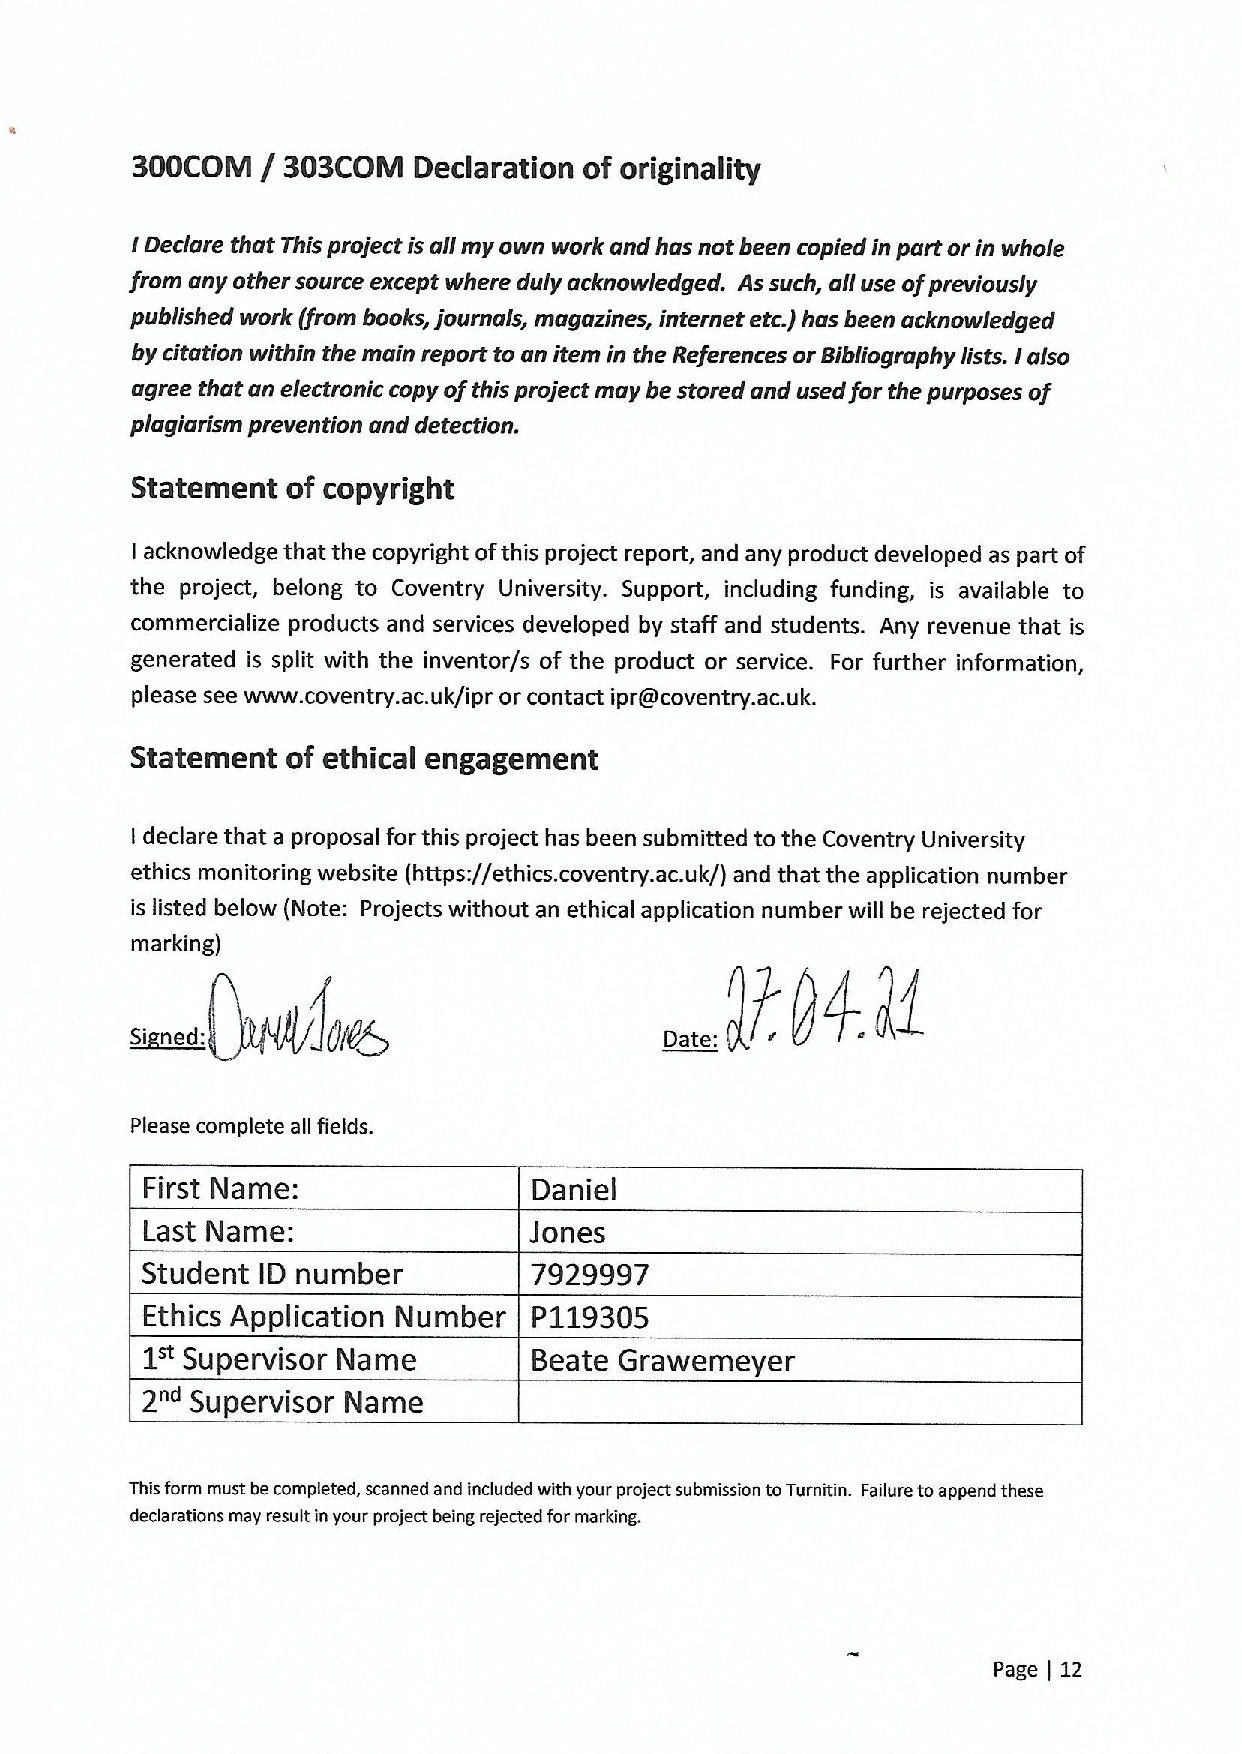
\includepdf[pages=-]{SER_Daniel_Jones_Declaration.pdf}
\begin{center}
	\vspace*{1cm}
	\Huge \textbf{A Speech Emotion Recognition Classifier to Aid Performance Review in Learning Environments} \\[1em]
	\vspace{5cm}
	\LARGE \textbf{Daniel G. Jones}
	\\
	\vspace{0.3cm}
	\large jonesd37@coventry.ac.uk
	\\
	\large Student ID: 7929997
	\\
	\vspace{3cm}
	\large Supervised by \textbf{Dr. Beate Grawemeyer}
	\\
	\vspace{0.3cm}
	\large ac7655@coventry.ac.uk
	\\
	\vspace{3cm}
	\large Submitted to the School of Computing, Engineering and Mathematics Coventry University
	\\
	April 2021
\end{center}
\newpage
\tableofcontents
\newpage
\section{Abstract}

Classifying human emotion from speech is a challenging problem that has the potential to benefit various fields in different ways. One such field is in learning environments, where the application of such technology could aid in matters such as performance review / analysis or in helping children with special needs, such as autism. In this project, a speech emotion classification model has been built and trained on the Ryerson Audio-Visual Database of Emotional Speech and Song (RAVDESS), and then deployed in the form of a graphical tool that analyses either pre-recorded audio or a live audio input and outputs the weighted predictions. The model has been developed using a 2-Dimensional Convolutional Neural Network (CNN) approach, where the training data is in the form of audio files converted into Mel Spectrograms. Through this approach, an exact prediction accuracy of 68.8\% has been achieved on an unseen test dataset, with further personalised tests yielding promising results.

\section{Acknowledgements}

With thanks to my project supervisor, Dr. Beate Grawemeyer, for the initial inspiration and constant support throughout the project.
\\

\noindent With thanks to my friend Céline Capelli of ETH Zürich for testing the application, providing useful audio data for testing, and for providing her unique perspective.
\\

\noindent With thanks to my partner Hannah Vogt of the Pädagogische Hochschule Zürich for her love, inspiration, motivation, and for imparting the insights of a primary school teacher. 
\\
\newpage

\section{Introduction}

It can be observed that technology has yet to make a significant contribution towards aiding performance review in learning environments and indeed learning environments on the whole. This can largely be attributed to the lack of effectiveness of the existing tools, whereby much of the information obtained is neither insightful nor particularly meaningful.
\\

\noindent Traditional approaches to the incorporation of technology in learning environments have tended to focus more on interactivity as opposed to analysis, which has resulted in a lack of progress in the areas of performance review, analysis, and overall utility (Cho et al. 2020). This is due in part to the complexity of such environments, with many subjective metrics and mediums that, at first glance, appear to be difficult to study and quantify.
\\

\noindent In this project, speech emotion has been identified and selected as a suitable metric for analysis. Speech emotion is a language agnostic metric that transcends many of the barriers posed by the more obvious metrics such as spoken / body language or facial expressions.
\\

\noindent Despite the many nuances of speech, such as tonality or pitch, there are clear patterns that can be derived from studying how emotions are conveyed (Angrick et al. 2019). A spectrogram is a visual representation of the spectrum of frequencies (in this case, the frequencies are converted to the mel scale) across a signal as a function of time. Consider the following mel spectrograms produced from two different male actors saying a short sentence in a blatantly angry and then sad manner.
\\
\\
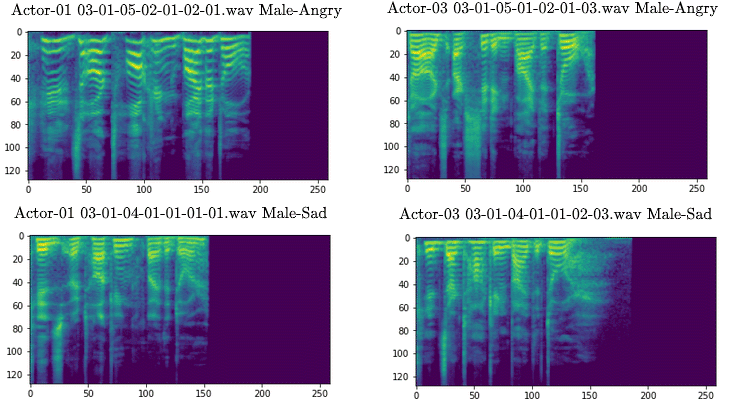
\includegraphics[width=14cm]{figure_1_spectrogram_comparison}

\noindent Figure 1 - spectrogram comparison.
\vspace{0.05cm}

\noindent Even from a macro perspective, it is possible to make out some visible similarities. Take for example the large circular shapes that can be made out from the two angry clips, or the distribution of the yellow (corresponding to pitch across the mel scale) lines in the sad clips. The spectrogram is represented by a matrix of values, which is where the vast, more subtle patterns can be identified and observed - making it an ideal candidate for a CNN approach.

\newpage

\noindent Prior to the increased popularity of machine learning, conventional methods for analysing and processing speech involved the usage of Gaussian Mixture Models (GMM) and Hidden Markov Models (HMM), both of which produced results that were simply too inaccurate to ever put into production (Sainath et al., 2013; Venkataramanan \& Rajamohan, 2019). The accessibility of machine learning techniques has lead to novel approaches such as the application of Recurrent Neural Networks (RNN) and CNNs, resulting in improved accuracy and introducing completely different approaches to the problem.
\\

\noindent In this paper, inspired by the notable success and improvements seen from the application of CNNs in particular, a relatively accurate classification model has been trained through applying CNNs to Mel Spectrogram representations of audio files. The Mel Spectrogram effectively allows us to transform the classification problem from the audio domain into the visual domain, where CNNs have demonstrated to excel. As previously shown in figure 1, there are many subtle patterns to be found in the data, but it is a difficult task to manually calculate and label these ourselves. Hence a deep learning approach, where the model learns to recognise and extract features itself, becomes a clear suitable choice.
\\

\noindent The final trained model has then been deployed into a general purpose graphical tool that can perform predictions across pre-recorded audio files or through recording on the fly. The graphical tool has been purposefully designed with simplicity in mind and with the intention of being easy to use and incorporate into learning environments.
\section{Research Objectives}
\begin{itemize}
\item To research, experiment, and develop an understanding with deep learning using industry standard frameworks.
\item To develop a plausible speech emotion classifier using state of the art techniques.
\item To deploy the speech emotion classification model into an accessible GUI application.
\item To assess the feasibility of such a tool for use in learning environments.
\end{itemize}

\section{Literature Review}

\subsection{\href{https://www.intechopen.com/books/social-media-and-machine-learning/automatic-speech-emotion-recognition-using-machine-learning}{Automatic Speech Emotion Recognition Using Machine Learning}}
Automatic Speech Emotion Recognition Using Machine Learning takes a comparative look at SER systems. The underlying method to extract and process the speech signals (using Mel-frequency cepstrum coefficients and modulation spectral features in conjunction with feature selection) remains the same whilst the machine learning paradigms differ. The paper first looks at a recurrent neural network approach and goes on to compare it against both multivariate linear regression and support vector machine approaches. The paper makes the claim that such approaches were selected due to their existing popularity in the field. 
\\

\noindent The initial criticism of the paper is that it fails to consider the CNN approach, despite its notable popularity and differences to the other methods. However, the paper is still concise and informative enough to warrant a full review. One positive quality that immediately stands out is how clear the information is presented, both in terms of looks and in use of language. An additional outstanding quality of this paper is the lack of pre-requisite knowledge required of the reader; many similar such papers assume at least a fundamental understanding and generally a lot more, whilst this paper describes most of the necessary knowledge required to grasp the content.
\\

\noindent The paper starts by explaining the importance behind SER technology, the main argument can be reduced to how effective and convenient it is to obtain information pertaining to the emotional state of an individual in comparison to other methods (such as facial expressions and physiological signals). This argument can be applied to the idea of using such technology in learning environments based on the documented effectiveness of the results in similar scenarios. The paper even uses learning environments as an example of a potential application of such technology; Kerkeni et al. (2019) state that ``a teacher can use SER to decide what subjects can be taught and must be able to develop strategies for managing emotions within the learning environment''.
\\

\noindent The authors then describe their system from a top-down perspective, this includes which emotions are in scope as well as the decision making process behind which algorithms are selected. It appears that the researchers were restricted by their datasets as to which emotions ended up in-scope. Whilst this does not affect the content of this particular paper, a more careful consideration will have to be made when applying this to learning environments (as per this project).
\\

\noindent Delving further into the paper, the authors describe how the different algorithms are applied to solve the problem, which is achieved by mathematical notation and descriptions of important variables. This is of course a necessity for such a paper, although the notation is clear enough for even those with weaker mathematical backgrounds to gain insight. The paper concludes by displaying and contrasting between the results obtained from the experiments; the main conclusion is that SER produces the best recognition results with a limited dataset whilst RNN performs better when a higher volume of data is available. Such results will prove vital when comparing against and assessing the effectiveness of our SER system.

\subsection{\href{https://www.mdpi.com/1424-8220/20/1/183/pdf}{A CNN-Assisted Enhanced Audio Signal Processing for Speech Emotion Recognition}}
Due to the notable omission of a CNN approach in the first reviewed paper, this paper has primarily been selected to gain practical insight into such an approach. The paper starts by defining the motivation behind it, using similar arguments to the previously reviewed paper. One particular area of interest is the point about ``extracting hidden information'', where Kwon (2020) refers to uncovering previously undetected, new information using a CNN approach. At first glance, it appears that the author looks at the issue more through the lens of human computer interaction (HCI), contrasting with the previous paper's theoretical approach.
\\

\noindent An immediate positive point of the paper is that it describes its approach clearly and in plenty of detail, though unlike the first paper, this paper requires the reader to possess fundamental knowledge concerning machine learning terminology and methods. The paper goes on to discuss the proposed methodology, which is essentially a model comprising of input layers (taking in 2D speech signal spectrograms), several convolutional layers flattened down, and two fully connected layers with the softmax classifier applied at the end. Compared to the first paper, this approach seems easier and requires a lot less pre-processing work applied to a given dataset (since the audio just needs transforming into a 2d spectrogram). The main downside to this paper is that it lacks technical and theoretical insight, providing only a single equation unrelated to the classifier itself.
\\

\noindent Cutting to the end results of the paper, given the clear lack of training applied to the model, the results achieved are not bad. Although lower than one might expect given some of the cutting-edge results achieved through CNNs on other projects; the lack of training surely impacts this. In conclusion, the paper has provided an insightful and inspiring approach to be considered for this project. As with the prior paper, the end results will be interesting to compare against in the end.

\subsection{\href{https://arxiv.org/pdf/1912.10458.pdf}{Emotion Recognition from Speech}}
Emotion Recognition from Speech has been monumental in aiding the architectural decisions taken for building the classifier used in this project. In the paper, the authors build and compare an assortment of comprehensive approaches to speech emotion recognition, comparing many of the industry standard methods, such as HMMs, Mel-frequency cepstrum coefficients (MFCCs), and CNNs. In particular, the authors find that a 4 layer model with batch normalisation and max pooling yields the highest accuracy across their dataset. The authors additionally discuss filtering and data processing techniques, such as applying Wiener filtering to the audio to help filter out noise. The paper provides an extremely useful framework of architectural decisions and comparisons that have proven very useful throughout the development of this project. 

\subsection{\href{https://files.eric.ed.gov/fulltext/EJ1194723.pdf}{Factors Affecting Technology Integration in the Classroom}}
This paper provides solid reasoning on the critical factors affecting the integration of technology in learning environments. The paper consists of 5 key reasons as to why classrooms benefit less from technology than many other environments: poor infrastructure, inadequate technology, lack of sufficient, effective professional development, low self-efficacy, and teacher perceptions. Each reason stated in the paper is insightful, but the points regarding inadequate technology and teacher perceptions are of the most relevance to the project. As previously mentioned, one of the goals of this project would be to put forth a valid and viable application of technology in learning environments (as to build some interest around the idea). Harrel \& Bynum (2018) state that teachers ``perceive the effort needed to learn the new technology and practicality of it as a significant consideration in whether they use it or not'', so in order for this to work, the educators must be convinced of the technology.

\subsection{\href{https://www.researchgate.net/profile/Ryan-Baker-2/publication/326217846_Modeling_Learners'_Cognitive_and_Affective_States_to_Scaffold_SRL_in_Open-Ended_Learning_Environments/links/5b560a4245851507a7c3f516/Modeling-Learners-Cognitive-and-Affective-States-to-Scaffold-SRL-in-Open-Ended-Learning-Environments.pdf}{Modeling learners' cognitive and affective states to scaffold SRL in open-ended learning environments}}
Whilst this paper largely covers an area unrelated to the project, the points regarding relationships between cognitive and affective states are interesting and will be of use to the analysis stage of the project. The paper goes on to describe an interesting correlation between two affective states, boredom and delight, and academic performance. As one might expect, an exposed state of boredom significantly decreases cognitive and subsequently academic performance, as documented by the paper. With these statistics in mind, prioritising the prediction of the states of boredom and delight from speech will be areas of particular interest to focus training the model on.
\section{Methodology}
Selecting the correct tools to tackle this project was challenging due to the many pros and cons of the existing frameworks available. Python was the obvious language of choice due to the massive amount of well documented machine learning libraries available. Had the dataset been larger however, Python and Python libraries would have been switched out for a lower level approach, using C++ for example, for efficiency. Initially PyTorch was selected as the deep learning framework of choice due to the pythonic syntax and therefore ease of use. Whilst an implementation could be made using PyTorch, the end model was fundamentally flawed. The documentation of PyTorch, especially for a beginner, is not the most clear; many parameters are not sufficiently explained and a lot of prior knowledge is assumed of the reader.
\\

\noindent Eventually PyTorch was switched for Keras and TensorFlow, with much more success. Whilst TensorFlow is not quite as elegant or lightweight as PyTorch, the documentation of the library is unmatched. Consequently, multiple successful deep learning models could then be built and deployed without much debugging required. Besides the machine learning libraries, the popular signal processing library Librosa was used to handle the processing and transformation of audio files. Librosa is well documented and can handle complicated audio transformations in only a few lines of code.

\section{Implementation}
The development of this project can be broken down into 5 key stages: dataset selection and comprehension, data processing, model architecture and training, testing, and finally, GUI development.
\subsection{Foreword}
A lot of the time spent on this project was spent prior to the key stages on personal development; this involved developing a theoretical and practical understanding of machine learning techniques. In particular, two LinkedIn Learning courses by Fernandes (2019) and Geitgey (2017) both played a large role in understanding how the technology worked at both the practical and theoretical levels. Once a core understanding was developed, consistent literature review of technical papers on speech emotion recognition helped to further shape the understanding towards the specific subject matter. 
\subsection{Dataset Selection and Comprehension}
Prior to embarking on any practical work for this project, consideration was made to the type of data that would be required to use for both testing and training the speech emotion classifier. One initial idea was to collect and sample our own data, but the ongoing global pandemic made this option infeasible. In general, the choices for such a dataset were highly limited, with only one option standing out in particular; The Ryerson Audio-Visual Database of Emotional Speech and Song (RAVDESS). RAVDESS is an open-source dataset (Kaggle, 2019) consisting of 1440 unique audio clips of actors speaking a sentence whilst blatantly conveying one emotion out of: calm, happy, sad, angry, fearful, surprise, and disgust.
\\

\noindent The selection of the RAVDESS dataset for this project meant that the emotions in scope were pre-determined, which, whilst not inherently detrimental, meant that prior work related to selecting the emotions best suited to the field of learning environments became redundant. Fortunately however, the more general emotions that had been selected prior were covered by the dataset with later developments showing that inferences about the more complicated in-scope emotions could be attained from the broad parent classes, as well as through studying the multi-class weighted predictions.

\noindent The dataset is already labelled such that the labels effectively describe the key content of the audio clip, as shown below in figure 2.
\\

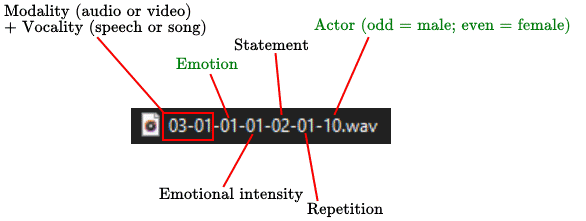
\includegraphics{figure_2_dataset_audio_example}
Figure 2 - an example audio file from the dataset; only the sections marked in green (emotion and gender) need to be taken into consideration.
\\


\noindent Since the dataset comes labelled and is well structured, the only administrative task was to extract the key labels from each of the audio files; this was achieved through the\code{get\_label\_RAVDESS} helper function (code in the Appendix). At first glance, the emotional intensity label may seem like a factor to consider, however, due to the limitations in terms of the size of the dataset, creating additional categories would only serve to make the classification more ambiguous.
\\

\noindent With regards to categorisation, this was initially set to include all of the default labelled emotions in the dataset, but later work revealed that this yielded worse results. The likely explanation for this is that the distribution of emotions throughout the dataset is uneven, meaning that not enough data can be studied to build viable connections. Upon further studying the minority emotions (calm and surprise), it was found that these could feasibly be converted in efforts to improve the neutral and happy emotion categorisation respectively. 
\\
\begin{center}
\begin{tabularx}{\textwidth}{ |X|X| }
\hline 
  \textbf{Original Label}  & \textbf{Converted Label} \\
  \hline
  Neutral & Neutral \\
  \hline
  Calm & \textbf{Neutral} \\
  \hline
  Happy & Happy \\
  \hline
  Sad & Sad \\
  \hline
  Angry & Angry \\
  \hline
  Fearful & Fearful \\
  \hline
  Disgust & Disgust \\
  \hline
  Surprised & \textbf{Happy} \\
  \hline
\end{tabularx}
\end{center}
Figure 3 - the final emotional labels used to train the model; in bold text are the conversions.
\\
\subsection{Data Processing}
Since the dataset comes in the form of labelled audio (.wav) files, the main task is to convert these to spectrograms, in particular mel spectrograms, that can later be used to train the model. Using the mel scale as opposed to the hertz scale is important when working with human audio; the mel scale is a scale derived from tests with human listeners, such that the scale of pitches is judged to be equal in distance from one another.
\\

\noindent The first task is converting the audio frequency from the hertz scale to the mel scale, this is given by the equation $m = 2595 \log_{10}\left(1 + \frac{Hz}{700}\right)$. Once this conversion is made, a mel spectrogram can be obtained from an audio signal by computing the squared magnitude of the Short-Time Fourier Transform (STFT) applied to a signal, substituting the frequency of the signal for the mel scale conversion. Finally, the mel spectrogram is scaled to decibel units according to $10 \times \log_{10}(mel \, spectrogram)$. This in turn corresponds to a weighted matrix, as in figure 4 below.
\\
\begin{center}
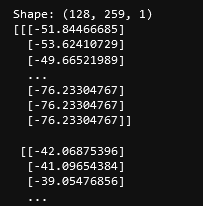
\includegraphics{figure_3_spectrogram_matrix}
\end{center}
Figure 4 - a log-scaled mel spectrogram obtained from an audio file from the dataset.
\begin{center}
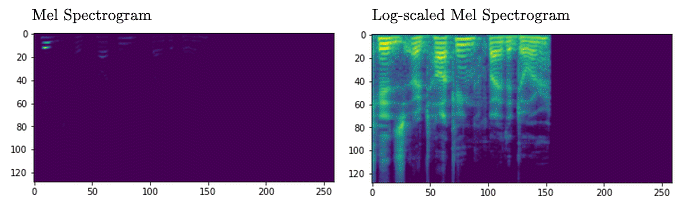
\includegraphics{figure_5_log_spectrogram}
\end{center}
Figure 5 - illustrating the importance of the decibel conversion.
\\

\noindent The last step of the data processing stage was creating the testing and training data through applying the labelling and spectrogram transformation functions to each audio file. The testing data was selected through a random sampling ($n = 180$) of assorted audio files containing all emotions in scope and all actors except actor 24. Actor 24 was excluded in an attempt to introduce some completely unknown data into the testing dataset.
\newpage
\subsection{Model Architecture \& Training}
The approach towards building the model involved researching existing models and simply experimenting with different variables. Research documented in the literature review, with particular regard to the paper by Venkataramanan \& Rajomohan (2019), showed that the convolutional neural network approach, applied to visualisations of signals, achieved by far the best results. Convolutional neural networks work by analysing discrete features within a tensor (which the spectrogram, as a matrix, can easily be converted to), which is then abstracted to a feature map that contributes towards the input of the next layer. The reason that this type of neural network is feasible for this project is due to the conversion of the audio signal to the spectrograph, essentially transferring the problem from the audio domain to that of the visual.
\\

\noindent The core architecture, consisting of 4 2-dimensional convolutional layers with max pooling, batch normalisation, dropout regularisation, and an exponential linear unit (ELU) activation function, therefore remained the same throughout the experiments. The Adam optimiser was selected due to the adaptive learning rate and categorical cross entropy was selected as the loss function (since the goal is to classify across multiple classes).
\\

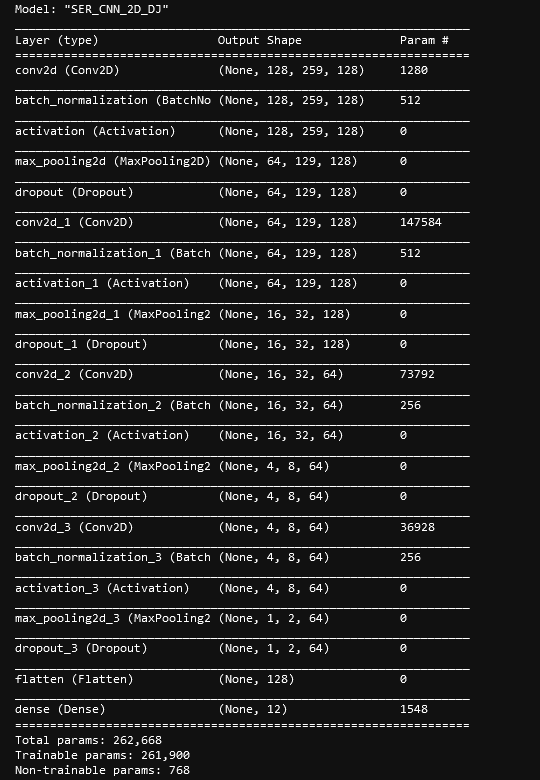
\includegraphics[width=10cm,height=14cm]{figure_6_model_visualisation}
\\

Figure 6 - summary of the complete speech emotion recognition model.
\\

\noindent Once the final design had been decided, the model was then trained several times using a multitude of different batch and epoch size combinations. The main goal was to strike a balance between optimisation and the over-fitting problem; 125 epochs at batch size 16 produced the most optimal results of the tests performed (including in terms of computational efficiency).
\\

\noindent The training steps and code can be viewed from the SER Classifier Jupyter Notebook with link in the appendix.
\subsection{Testing}
After the final model was trained, the test dataset was loaded and tested blindly on the model, yielding 180 predictions. The categorical accuracy across this dataset was 68.88\%, which is a comparatively high score. Whilst the accuracy is most certainly inflated due to the similarities of the test dataset (all of the speakers being North American actors speaking English and saying similar sentences), the results are still impressive considering both the lack of training data and the fact that the majority of the test data consisted of actors that had not been used to train the model at all. 
\begin{center}
\begin{tabularx}{\textwidth}{ |X|X| }
\hline 
  \textbf{Actual value} & \textbf{Prediction} \\
  \hline
  22. female sad & 22. female neutral \\
  \hline
  28. female angry & 28. female neutral \\
  \hline
  45. female disgust & 45. male sad \\
  \hline
  72. male happy & 72. female happy \\
  \hline
  80. male sad & 80. male neutral \\
  \hline
  100. male fearful & 100. male happy \\
  \hline
  152. female angry & 152. male angry \\
  \hline
\end{tabularx}
\end{center}
Figure 7 - a sample of the incorrect predictions, showing reasonable mistakes (i.e. emotional similarity or right emotion; wrong gender). \textit{Values taken from SER\_Classifier notebook}.
\\

\noindent After the model had been tested on sample data from the same dataset, the next step was to test it on completely unique audio. The main source of this audio was from myself and from family and friends. From personal tests using my own voice, the results yielded were positively surprising. In particular, the model had shown to have learned the negative emotions particularly well; correctly predicting male anger for each of the sample clips (included in the GitHub repository). What was also impressive was that the model wasn't just predicting the correct emotion with a slight edge over the other categories; the model would predict anger with over 90\% accuracy over the other categories (with male disgust, female anger, and male sad often taking up the remainder of the prediction for this category).
\newpage
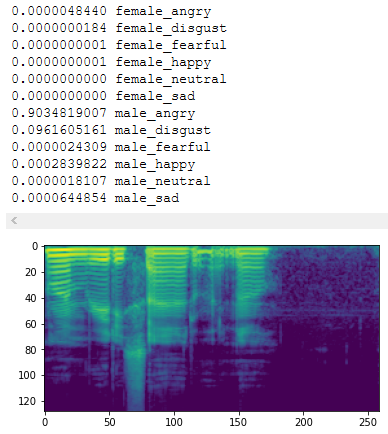
\includegraphics[width=7cm, height=6cm]{figure_8_personal_prediction}
\\
Figure 8 - output predictions using an audio clip of myself talking angrily, available through the appendix.
\\

\noindent A particularly interesting test was conducted using a friend of mine with diagnosed Asperger's syndrome who notably struggles to perceive the emotions of others. For the test, she was asked to send some audio clips of herself conveying an impression of the various emotions in scope. The overall accuracy initially seemed poor, with some predictions failing to even fit the binary classification of positive/negative. Upon looking further into this and analysing the audio files together, we agreed that actually she herself had misclassified emotions that the predictions from the model were more reflective of. 
\begin{center}
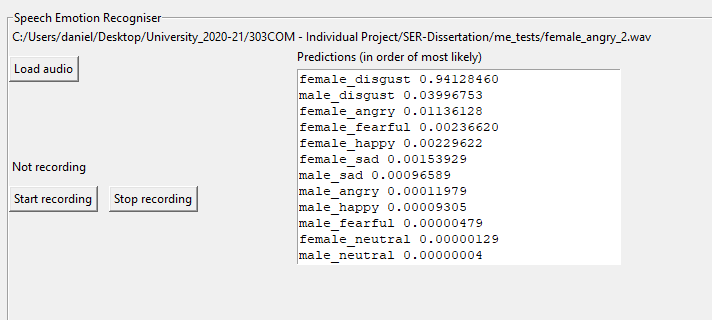
\includegraphics[width=16cm, height=9cm]{figure_9_autism}
\end{center}
Figure 9 - an example of one of the tests on a friend with autism who had herself misclassified the audio (and a preview of the GUI tool).
\\

\noindent The model was also tested on German and Swiss German language audio to check for any variance in results when straying from English. In these tests, sentences were said exclusively in the respective language whilst an emotion from the list was conveyed. The model generally performed well, correctly predicting the emotion for angry / sad / disgust but made some errors on the positive emotions tested. It is worth noting that in the cases where it failed, the target emotion was always within at least the top 5 prediction classes.
\subsection{GUI Development}
Once the model had been developed, tested, and evaluated, the final step of this project was to deploy the model into a functional tool for end-users. The primary objective of the tool was that a user with next to no technical background could easily obtain results from the model without having to write code or tweak files. The core functionality of the tool was relatively easy to determine; the user should be able to analyse pre-recorded audio and should be able to record audio directly so that the audio would be analysed and the results clearly visible. Since accessibility was an important factor, the tool was developed with simplicity and efficiency in mind. To achieve this, the tool was built natively within Python using Tkinter and with minimal libraries / graphics. The tool at first glance is shown in figure 10 and figure 9 shows a working example.
\begin{center}
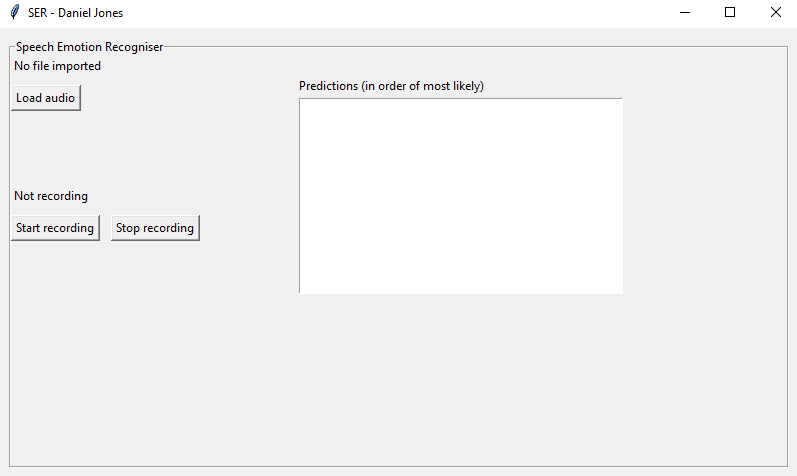
\includegraphics[width=16cm, height=9cm]{figure_10_finished_tool}
\end{center}
Figure 10 - The tool upon execution, showing the two key functions as buttons.
\section{Evaluation}
The end result of this project is both a promising speech emotion recognition classifier (by account of the tested accuracy, both on the test dataset, and according to personal tests) and a fully functional tool that can be used by end users in a variety of different environments. In this section, I will relate both the successes and failures of the project back to the original research objectives as defined in the project proposal document under the ``Primary Research Plan''.
\subsection{Research Objectives}
The first and primary research objective was to create a capable speech emotion classifier based on current literature. By account of the various tests and experiments, I believe that a viable model has been successfully built and trained utilising methods that produce competitive results. This has been achieved through constant literature review and through personal research on theoretical machine learning and machine learning best practices. The end model and all of the associated work contained in the notebook should serve as a clear and concise approach to tackling the problem, demonstrating what works and what could be improved. 
\\

\noindent The next research objective was to improve and modify the model through conducting formal tests and through conducting research in learning environments. Unfortunately this objective was unsuccessful, as these tests could not take place. However, I do believe that the end product is in a capable condition, where it could easily be picked up from where it is currently left to be further developed. Since the deployment of the product and core architecture are taken care of, this would be only be a matter of additional data collection, processing, and re-training, which are comparatively inexpensive. 
\\

\noindent The final research objective, to create a tool that could be used within learning environments by end users has, I believe, been achieved. A GUI tool has been produced that is very lightweight, yields results quickly, and requires little dependencies once deployed. The GUI is intentionally simple, and through testing with a user with autism, has proven to add at least some unique and useful insights. With regards to the final GUI, since it is intentionally simple and lightweight (according to research regarding technology in learning environments), I do not believe that it could be further improved without further adjusting the model or gaining real world feedback from learning environments.
\\

\noindent Overall I believe that good work has been made in achieving the research objectives, whilst not achieving them all perfectly, progress has been made and the end result is in a particularly nice stage that I intend to personally pick up, carry on with, and develop further in a future project. 

\newpage
\section{Discussion and Conclusion}
The project was originally structured around three key pillars; building a speech emotion recognition classifier, building an accessible tool to utilise the classifier, and testing it within learning environments to document the findings. The idea behind this structure was that, upon completion of any stage, there would at least be something to document and contribute back to the field. Unfortunately, the third stage of the project was not able to take place due largely to the global pandemic, but also due to a personal underestimation of the length of time required to even begin understanding the fields of signal processing and machine learning. However, the amount of personal development and new knowledge I have been able to gain through undertaking this project have been of immeasurable value to me.
\\

\noindent The main strength of the project is the final product itself, which I believe offers a functionality that is, in some cases, insightful enough to be used as is. For example, the tests performed with my friend with autism directly show that the tool can offer useful insights previously unobtainable. Furthermore, the model architecture and trained model both provide a useful checkpoint that could easily be enhanced further through additional data volume. If nothing else, I believe that the model and final application developed alongside this project provide a clear and well documented framework to anyone looking to enter speech emotion recognition or gain a head start in developing their own approach. 
\\

\noindent Was I to embark on this project from the beginning again, I would certainly choose less ambitious targets and goals. The core development of the project took far more time than originally anticipated, which I should have taken into consideration when planning the project. I would also change my approach to form a better foundation before starting on the practical work, because through doing this, a lot of debugging time could have been saved and concentrated elsewhere, resulting in a better overall project. 
\\

\noindent Despite the lack of new research linked to the usage of the tool in learning environments, the tool itself has been successfully developed and documented, and could easily be picked up from where it has been left off to continue further work with the project. Combining this with the vast amount I have learned makes this project a huge personal success. 
\newpage

\section{Project Management}
A waterfall-like project management methodology, namely IPERKA, was selected due to the structure of the project (as discussed in the \textbf{Discussion} section) and because of prior work experience using the methodology. IPERKA stands for ``Informieren, Planen, Entscheiden, Realisieren, Kontrollieren, and Auswerten'' which translates to ``informing, planning, deciding, implementing, controlling, and evaluating''. The methodology places lots of importance on project planning via the first three stages, which I felt was beneficial here due to the lack of experience prior to commencing the project.
\\

\noindent Regular weekly meetings with my supervisor were organised and held over Microsoft Teams each week to discuss both ideas, problems, and progress. I found these meetings extremely useful as they motivated me to stay on track, organise my thoughts, and discuss the feasibility of ideas. I dedicated approximately 2 days each week (requiring more particularly towards the end of the project) towards working on the project. An example of the notes taken during these sessions is shown below.
\begin{center}
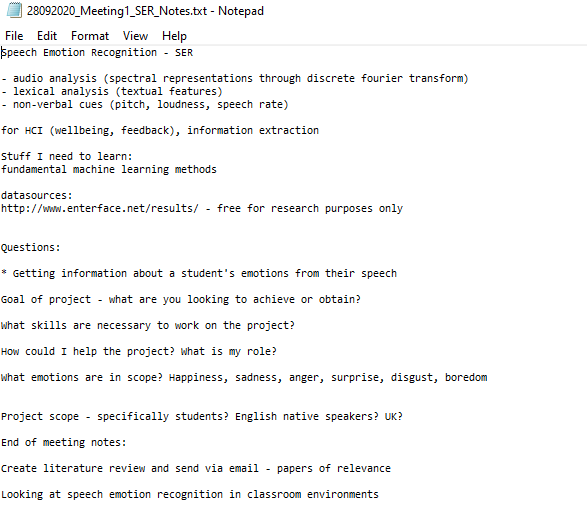
\includegraphics[width=15cm, height=12cm]{figure_11_notes}
\end{center}
Figure 11 - an example of notes taken from the very first meeting with my supervisor, discussing initial requirements and ideas.
\newpage
\subsection{Gantt Chart}
To help stick to a schedule and plan, I worked predominantly according to a Gantt chart, drafted in the early stages of the project. Whilst I wasn't able to exactly follow the Gantt chart, the structure and clarity provided by it proved to be worthwhile throughout the project, highlighting a clear path towards the final goals.
\\

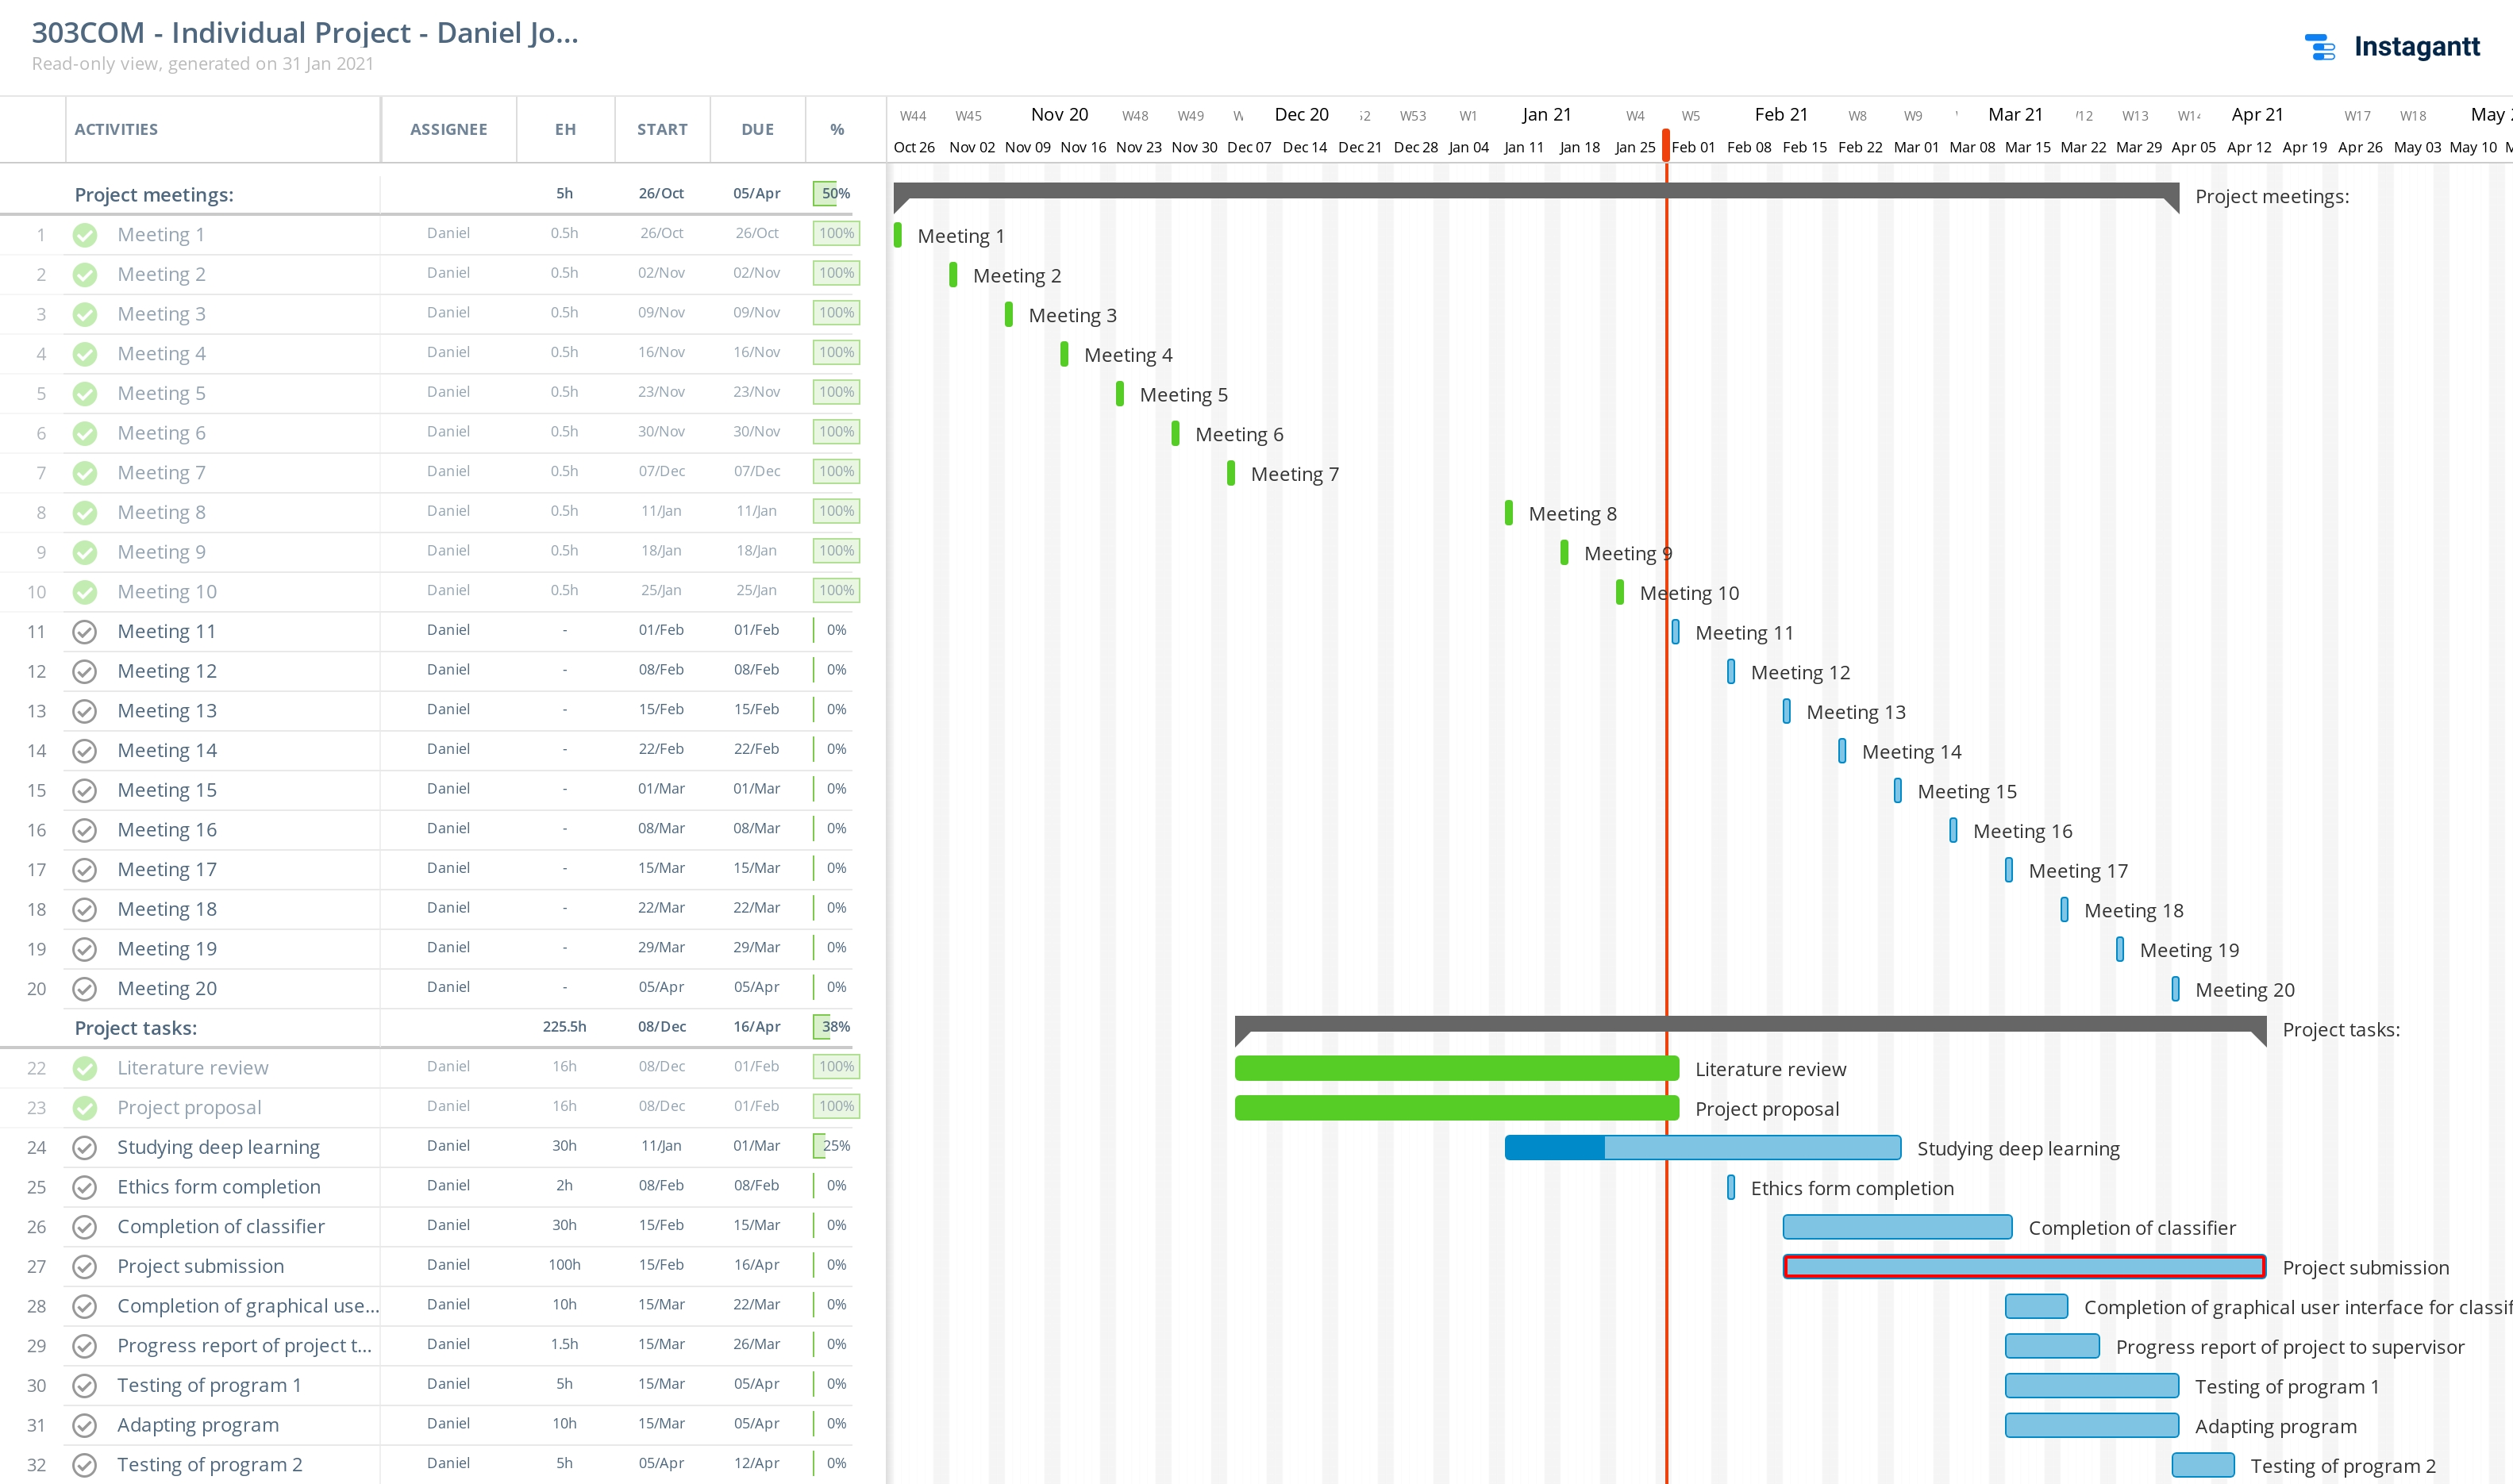
\includegraphics[width=18cm, height=12cm]{Daniel_Jones_Gantt_Chart}
Figure 12 - A screen-shot taken from the Gantt chart showing meeting plans and tasks to be completed.
\\
\noindent \href{https://i.imgur.com/9tchO4N.jpg}{\color{blue}\textbf{Link to full size image}}
\\
\noindent \href{https://app.instagantt.com/shared/s/PdaKZZeApqszVu1eftjC/latest}{\color{blue}\textbf{Link to latest edition of the chart}}
\subsection{Presentation}
Several progress presentations took place throughout the project life-cycle, particularly when milestone accomplishments (such as finishing the model and the GUI) had been accomplished. In the first presentation, a now redundant feature was demonstrated with positive feedback and with nothing to add or change. In the second presentation, the primary model architecture was demonstrated, receiving positive feedback. In the second presentation, the main comment was on the emphasis of deploying the model into a GUI tool with some discussion about the core functionality of the tool. In the final presentation, the GUI tool and the core functionality of the tool was presented through demonstrating the recognition capabilities using my own voice along with some pre-recorded clips. The feedback was completely positive with nothing to add or change.
\subsection{Consideration of social, legal, professional, and ethical issues}
The potential social, legal, professional, and ethical issues that could develop from this project must certainly be paid careful attention to. The implications of a tool that can predict emotions from speech could have negative implications if careful disclaimers are not disclosed regarding the project. That is to say that, whilst emotion can be predicted with a relatively high accuracy, the key word is ``predicted''; the model of course is prone to errors and even results that clearly do not make sense. An example of misuse would involve any attempt to use the project to draw absolute conclusions about speech emotion, such that the results would then influence additional decision making. Contained within the project repository is a disclaimer highlighting some of the key points (what the tool is and isn't) along with a fair usage license (MIT License). Essentially, the tool is a novel device that is made exclusively with guidance in mind. If the tool can be useful, for example to users with relevant disabilities or within learning environments, then it should only be used to prompt (through the range of the predictions) or to offer an alternative perspective.
\begin{center}

\includegraphics[width=15cm, height=2cm]{figure_12_disclaimer}
\end{center}
Figure 12 - the disclaimer included within the README.md file of the associated GitHub repository.
\newpage

\section{References}

\begin{itemize}
\item Cho, V., Mansfield, K. C., Claughton, J. (2020). The past and future technology in classroom management and school discipline: A systematic review. \textit{Teaching and Teacher Education, 90}, 103037. \href{https://doi.org/10.1016/j.tate.2020.103037}{https://doi.org/10.1016/j.tate.2020.103037}

\item Angrick, M., Herff, C., Johnson, G., Shih, J., Krusienski, D., Schultz, T. (2019). Interpretation of convolutional neural networks for speech spectrogram regression from intracranial recordings. \textit{Neurocomputing}, 342, 145-151.

\item Sainath, T. N., Mohamed, A. R., Kingsbury, B., Ramabhadran, B. (2013). Deep convolutional neural networks for LVCSR. In \textit{2013 IEEE international conference on acoustics, speech and signal processing} (pp. 8614-8618). \tab \href{https://ieeexplore.ieee.org/abstract/document/6639347}{https://ieeexplore.ieee.org/abstract/document/6639347}

\item Venkataramanan, K., Rajomohan, H. R. (2019). Emotion Recognition from Speech \textit{arXiv preprint arXiv:1912.10458}. \href{https://arxiv.org/pdf/1912.10458.pdf}{https://arxiv.org/pdf/1912.10458.pdf}

\item Kerkeni, L., Serrestou, Y., Mbarki, M., Raoof, K., Mahjoub, M.A., Cleder, C. (2019). Automatic Speech Emotion Recognition Using Machine Learning. In \textit{Social media and machine learning}. IntechOpen. \href{https://doi.org/10.5772/intechopen.84856}{https://doi.org/10.5772/intechopen.84856}

\item Kwon, S. (2020). A CNN-assisted enhanced audio signal processing for speech emotion recognition. \textit{Sensors 20(1), 183}. \href{http://doi.org/10.3390/s20010183}{http://doi.org/10.3390/s20010183}

\item Harrell, S., Bynum, Y. (2018). Factors affecting technology integration in the classroom. \textit{Alabama Journal of Educational Leadership}, 5, 12-18

\item Lim, W., Jang, D., Lee, T. (2016). Speech emotion recognition using convolutional and recurrent neural networks. In \textit{2016 Asia-Pacific signal and information processing association annual summit and conference (APSIPA)} (pp. 1-4). IEEE. \href{http://www.apsipa.org/proceedings_2016/HTML/paper2016/137.pdf}{paper2016.pdf}

\item Munshi, A., Rajendran, R., Ocumpaugh, J., Biswas, G., Baker, R. S., Paquette, L. (2018). Modeling learners' cognitive and affective states to scaffold SRL in open-ended learning environments. In \textit{Proceedings of the 26th conference on user modeling, adaptation and personalization}(pp. 131-138). \tab \href{https://doi.org/10.1145/3209219.3209241}{https://doi.org/10.1145/3209219.3209241}

\item Fernandes, J. (2019, October). \textit{PyTorch Essential Training: Deep Learning} [Video]. LinkedIn. \\ \href{https://www.linkedin.com/learning/pytorch-essential-training-deep-learning/welcome?u=2039756}{https://www.linkedin.com/learning/pytorch-essential-training-deep-learning/}

\item Geitgey, A. (2017, August). \textit{Building and Deploying Deep Learning Applications with TensorFlow} [Video]. LinkedIn. \href{https://www.linkedin.com/learning/building-and-deploying-deep-learning-applications-with-tensorflow/what-is-tensorflow?u=2039756}{https://www.linkedin.com/learning/building-and-deploying-deep-learning-applications-with-tensorflow/what-is-tensorflow}

\item Kaggle. (2019). \textit{RAVDESS Emotional speech audio}\\\href{https://www.kaggle.com/uwrfkaggler/ravdess-emotional-speech-audio}{https://www.kaggle.com/uwrfkaggler/ravdess-emotional-speech-audio}
\end{itemize}
\section{Appendix}
\begin{itemize}

\item \href{https://github.com/danielj0nes/SER-Dissertation}{\textbf{https://github.com/danielj0nes/SER-Dissertation}} - GitHub repository containing all of the referenced files, such as the Jupyter Notebook SER\_Classifier.ipynb (where the model was built) and SER\_Application.py where the model was deployed. The repository also contains all of the personal audio files using for testing and documenting results, the source code and images for this document, and will be made available from the 30th of April 2021 18:00 GMT (according to final submission deadline).

\item \href{https://www.kaggle.com/uwrfkaggler/ravdess-emotional-speech-audio}{\textbf{RAVDESS Emotional speech audio}} - Primary testing and training data used in the project (available for download via the link).

\end{itemize}

\end{document}